\documentclass[11pt,a4paper]{article}

\usepackage[spanish,es-nodecimaldot]{babel}
\usepackage[T1]{fontenc}
\usepackage{lmodern}
\usepackage{microtype}
\usepackage{geometry}
\usepackage{amsmath,amssymb}
\usepackage{booktabs}
\usepackage{tabularx}
\usepackage{graphicx}
\usepackage{float}
\usepackage{xcolor}
\usepackage{tikz}
\usetikzlibrary{arrows.meta,positioning}
\usepackage{enumitem}
\usepackage{fancyhdr}
\usepackage[hidelinks]{hyperref}

\geometry{margin=22mm,headheight=14pt}
\definecolor{navy}{HTML}{17324D}
\definecolor{blue}{HTML}{2C6E9B}
\definecolor{cyan}{HTML}{DCEEF5}
\definecolor{green}{HTML}{24765A}
\definecolor{softgray}{HTML}{F3F5F7}
\hypersetup{colorlinks=true,linkcolor=blue,urlcolor=blue}
\setlength{\parindent}{0pt}
\setlength{\parskip}{6pt}
\setlist[itemize]{leftmargin=5mm,itemsep=2pt,topsep=3pt}
\pagestyle{fancy}
\fancyhf{}
\lhead{\textcolor{navy}{Koopman--JEPA}}
\rhead{\textcolor{navy}{Informe final}}
\cfoot{\thepage}

\newcommand{\resultbox}[1]{%
  \begin{center}
  \fcolorbox{green}{cyan}{\parbox{0.90\textwidth}{\centering\bfseries\color{navy}#1}}
  \end{center}}

\begin{document}

\begin{center}
  {\Huge\bfseries\color{navy} Koopman--JEPA}\par
  \vspace{3mm}
  {\Large ¿Puede un JEPA aprender operadores dinámicos no triviales?}\par
  \vspace{2mm}
  {\large Informe final del experimento controlado}\par
  \vspace{2mm}
  {\small Septiembre de 2026}
\end{center}

\resultbox{Sí, bajo los datos y la receta estudiados: el predictor identifica
tres operadores en 10/10 seeds por condición y sigue una familia continua con
MAE espectral 0.027. Esto demuestra posibilidad, no necesidad ni superioridad:
DMD crudo y PCA+DMD también resuelven este dataset.}

\section{Pregunta}

Buscamos una representación $z_t=f_\theta(x_t)$ y un predictor lineal $M$ tales
que
\[
M z_t\approx z_{t+1}.
\]
Si $\psi(r_t)$ describe la fase verdadera, $K$ es su operador y el encoder
aprende $z\approx A\psi$, la prueba relevante es
\[
\boxed{MA\approx AK}.
\]
No exigimos $M=K$: el encoder puede elegir otra base. Medimos tanto la acción
de $M$ como su espectro restringido al span activo de los centroides latentes.

\section{Datos y control causal}

El estado oculto tiene cuatro fases $r\in\{0,1,2,3\}$. Cada fase genera una
ventana de longitud 128:
\[
x_t[\tau]=a_t\,s_{r_t}(\tau-\delta_t)+b_t+\epsilon_{t,\tau},
\]
con amplitud, offset, jitter temporal y ruido independientes. Los mismos bancos
de ventanas actuales y futuras se reutilizan en todas las condiciones; sólo
cambia el emparejamiento temporal.

\begin{center}
\begin{tabularx}{\textwidth}{@{}lXl@{}}
\toprule
\textbf{Dinámica} & \textbf{Transición} & \textbf{Espectro activo}\\
\midrule
Estática & $r_{t+1}=r_t$ & $\{1,1,1\}$\\
Cíclica & $r_{t+1}=r_t+1\pmod 4$ & $\{-1,i,-i\}$\\
Independiente & fase futura uniforme & $\{0,0,0\}$\\
\bottomrule
\end{tabularx}
\end{center}

Por seed y condición usamos 1024 pares de entrenamiento y 256 de validación.
La prueba principal repite 10 seeds. La auditoría verifica marginales idénticos,
transiciones correctas y fase perfectamente decodificable; una ventana aislada
no revela a qué dinámica pertenece.

\section{Arquitectura y supuestos}

\begin{center}
\resizebox{\textwidth}{!}{%
\begin{tikzpicture}[
  node distance=7mm and 8mm,
  box/.style={draw=navy,rounded corners,fill=softgray,align=center,
              minimum height=10mm,text width=33mm,font=\small},
  latent/.style={draw=blue,rounded corners,fill=cyan,align=center,
                 minimum height=9mm,text width=20mm,font=\small},
  loss/.style={draw=green,rounded corners,fill=green!10,align=center,
               minimum height=9mm,text width=24mm,font=\small},
  arrow/.style={-{Latex[length=2mm]},thick,draw=navy}
]
\node[box] (xt) {ventana actual\\$x_t\in\mathbb{R}^{1\times128}$};
\node[box,right=of xt] (online) {encoder online\\Conv $1\to16\to32$\\Flatten, Linear $\to3$};
\node[latent,right=of online] (zt) {$z_t\in\mathbb{R}^3$};
\node[box,right=of zt] (pred) {predictor lineal\\$M\in\mathbb{R}^{3\times3}$\\sin bias};
\node[latent,right=of pred] (zhat) {$\widehat z_{t+1}$};
\node[box,below=20mm of xt] (xnext) {ventana futura\\$x_{t+1}$};
\node[box,right=of xnext] (target) {encoder target\\misma CNN\\stop-gradient};
\node[latent,right=of target] (zplus) {$z^+_{t+1}$};
\node[loss,right=22mm of zplus] (mse) {MSE predictiva};
\draw[arrow] (xt)--(online);
\draw[arrow] (online)--(zt);
\draw[arrow] (zt)--(pred);
\draw[arrow] (pred)--(zhat);
\draw[arrow] (xnext)--(target);
\draw[arrow] (target)--(zplus);
\draw[arrow] (zhat)--(mse);
\draw[arrow] (zplus)--(mse);
\draw[arrow,dashed] (online.south) -- node[left=2mm,font=\scriptsize]{EMA 0.90} (target.north);
\end{tikzpicture}}
\end{center}

Se entrena 60 épocas con AdamW. El predictor usa learning rate $4\times$ mayor;
el encoder se congela tras la época 3 y el target se actualiza por EMA. La loss
agrega regularización de media, varianza y covarianza para evitar colapso.

La dimensión latente 3 coincide con el rango verdadero y el freeze temprano
estabiliza el ajuste de $M$. Ambos son supuestos del resultado, no propiedades
generales de JEPA.

\section{Resultado principal: tres operadores}

Para cada candidato $d$ calculamos
\[
E_d=\frac{\lVert MA-AK_d\rVert_F}{\lVert A\rVert_F}.
\]
También comparamos los autovalores de $M$ en el span activo. El criterio fijado
antes de correr fue al menos 8/10 seeds correctas por acción y por espectro.
La loss no participa en esta decisión.

\begin{center}
\begin{tabular}{@{}lrrrr@{}}
\toprule
\textbf{Dinámica} & \textbf{Acción} & \textbf{Espectro} & \textbf{Error} & \textbf{Margen}\\
\midrule
Estática & 10/10 & 10/10 & 0.142 & 0.806\\
Cíclica & 10/10 & 10/10 & 0.068 & 0.877\\
Independiente & 10/10 & 10/10 & 0.015 & 0.981\\
\bottomrule
\end{tabular}
\end{center}

\begin{figure}[H]
\centering
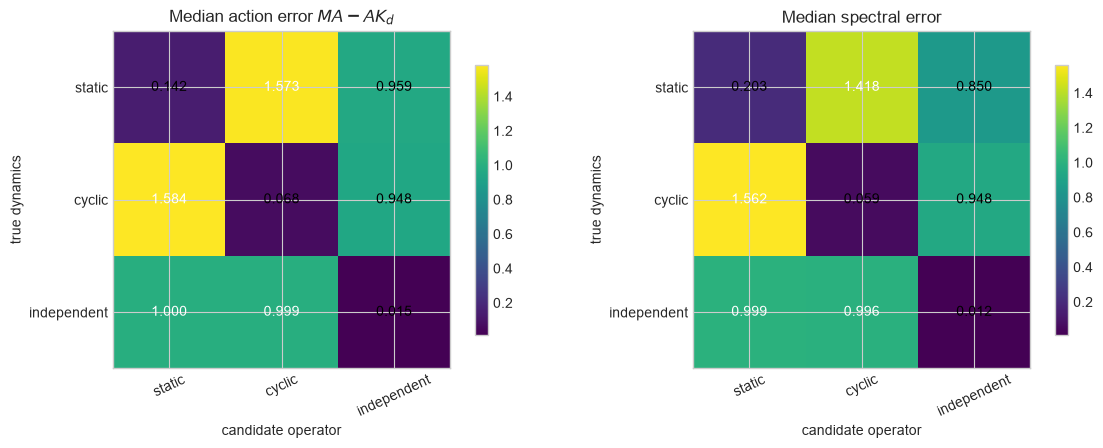
\includegraphics[width=\textwidth]{figures/three_dynamics_operator_identification.png}
\caption{Error mediano contra cada candidato. Cada fila usa los mismos
marginales observables y un pairing distinto. La diagonal es mínima tanto por
acción como por espectro.}
\end{figure}

\begin{figure}[H]
\centering
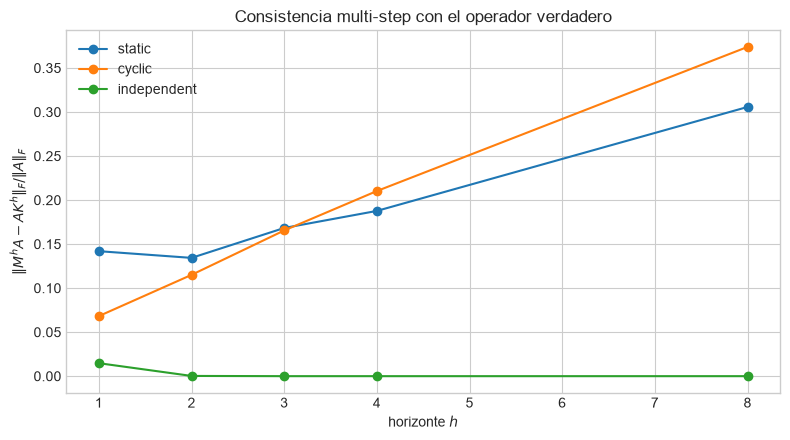
\includegraphics[width=0.86\textwidth]{figures/three_dynamics_rollout.png}
\caption{Error $\lVert M^hA-AK^h\rVert_F/\lVert A\rVert_F$. La identificación
a un paso es clara; en estática y cíclica el error se acumula con el horizonte.}
\end{figure}

\section{Generalización a una intensidad continua}

Interpolamos entre el ciclo $C$ y una transición uniforme $U$:
\[
P_\rho=\rho C+(1-\rho)U,
\qquad K_\rho=\rho C,
\qquad \operatorname{spec}(K_\rho)=\rho\{-1,i,-i\}.
\]

\begin{center}
\begin{tabular}{@{}rrrr@{}}
\toprule
$\boldsymbol{\rho}$ & \textbf{Acción} & \textbf{Espectro} & \textbf{Módulo mediano}\\
\midrule
0.00 & 10/10 & 10/10 & 0.016\\
0.25 & 10/10 & 10/10 & 0.239\\
0.50 & 9/10 & 9/10 & 0.476\\
0.75 & 8/10 & 8/10 & 0.718\\
1.00 & 7/10 & 7/10 & 0.948\\
\bottomrule
\end{tabular}
\end{center}

\begin{figure}[H]
\centering
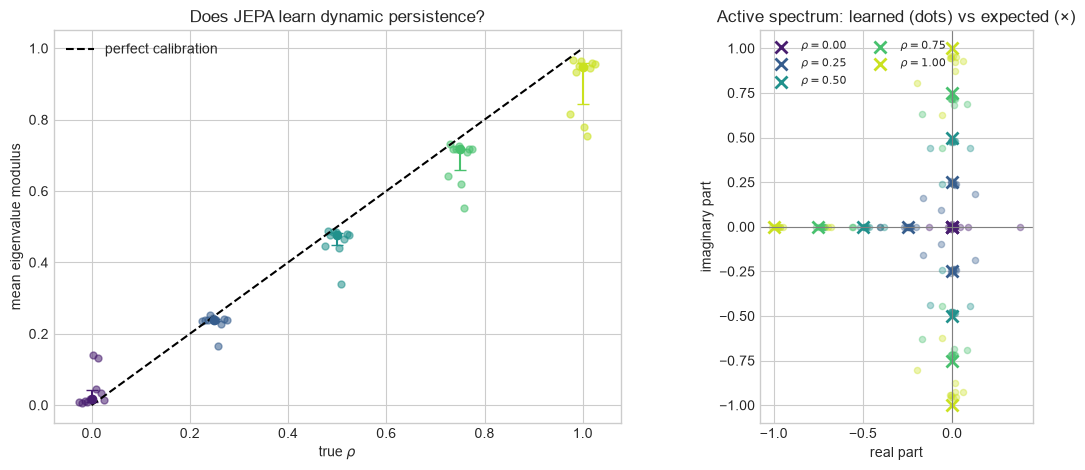
\includegraphics[width=\textwidth]{figures/decay_spectral_calibration.png}
\caption{Izquierda: módulo espectral aprendido contra $\rho$. Derecha:
autovalores esperados y aprendidos en el plano complejo.}
\end{figure}

La calibración continua tiene MAE 0.027, pendiente 0.937, intercepto 0.011 y
$R^2=0.9998$. El criterio discreto de 8/10 en cada nivel no pasa porque
$\rho=1$ queda en 7/10: algunas seeds eligen el nivel vecino por un sesgo
contractivo. Se conservan ambas lecturas sin crear un nuevo umbral post-hoc.

\section{¿JEPA es lo que hace el trabajo?}

Comparamos siete métodos sobre la misma familia continua. Esta tabla corresponde
a una sola seed de validación: contextualiza el mecanismo, pero no es una
comparación confirmatoria multiseed.

\begin{center}
\small
\begin{tabularx}{\textwidth}{@{}Xrrr@{}}
\toprule
\textbf{Método} & \textbf{MAE espectral} & \textbf{MAE acción} & \textbf{Pendiente}\\
\midrule
Oracle de fase + OLS & 0.000 & 0.000 & 1.000\\
Ventana cruda + DMD & 0.022 & 0.020 & 0.949\\
PCA-3 + DMD & 0.011 & 0.011 & 0.975\\
CNN aleatoria + DMD & 0.299 & 0.137 & 0.391\\
CNN supervisada + DMD & 0.012 & 0.011 & 0.968\\
JEPA + $M$ aprendido & 0.197 & 0.103 & 0.435\\
Encoder JEPA + DMD post-hoc & 0.029 & 0.026 & 0.952\\
\bottomrule
\end{tabularx}
\end{center}

JEPA mejora a la CNN aleatoria, pero DMD crudo y PCA+DMD obtienen menor error.
El encoder JEPA con DMD post-hoc mejora mucho al predictor entrenado, lo que
sitúa el principal cuello de botella en la optimización conjunta de $M$. Este
dataset no permite afirmar que JEPA sea necesario ni superior.

\section{Conclusión exacta}

\textbf{La evidencia sí apoya} que este JEPA puede representar una dinámica no
trivial y que su espectro responde casi linealmente a la persistencia dinámica,
bajo la arquitectura, dimensión latente, freeze, EMA, regularizadores y datos
documentados.

\textbf{La evidencia no apoya} recuperación general de Koopman, superioridad
sobre métodos lineales, robustez fuera de distribución ni independencia de la
receta. La comparación de baselines quedó en una seed de validación y su
held-out no se abrió. El estudio se cierra con este alcance; no se atribuye al
experimento una conclusión que no fue medida.

\section*{Reproducibilidad}

El flujo completo está reducido a cinco notebooks ejecutados en
\path{notebooks/}. Las cuatro configuraciones están en \path{configs/}, el
diseño consolidado en \path{docs/EXPERIMENT.md} y la implementación reutilizable
en \path{src/koopman_jepa/}. Los tests verifican datos, álgebra, entrenamiento y
outputs versionados.

\end{document}
